\usetikzlibrary{patterns}
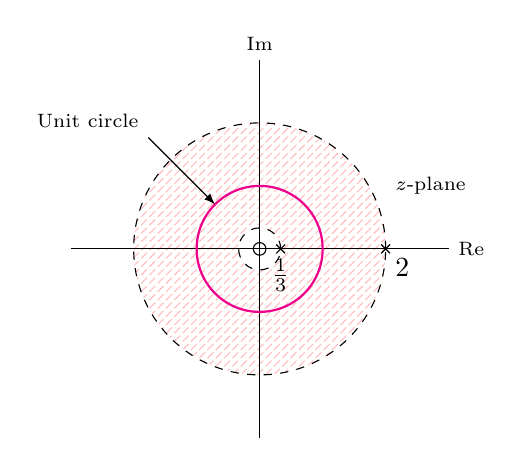
\begin{tikzpicture}[scale=0.8]
    \def\pole{++(135:0.1) -- ++(-45:0.2) ++(135:0.1) -- ++(45:0.1) -- ++(-135:0.2) +(45:0.1)}
    \def\zero{circle (0.1)}
    	\begin{scope}
     		%\path [pattern color=pink, pattern=north east lines] (-3, -3)  rectangle (3, 3);
     		\draw [dashed, pattern color=pink, pattern=north east lines] (0,0) circle (2);
     		\draw [dashed, fill=white] (0,0) circle (1/3);     		
	\end{scope}

    \draw (-3, 0) -- (3,0) node[anchor=west] {\scriptsize $\mathrm{Re}$};
    \draw (0, -3) -- (0,3) node[anchor=south] {\scriptsize $\mathrm{Im}$};
    %\pause
    \draw[thick, magenta] (0,0) circle (1);
    \draw [latex-] (0,0) ++(135:1) -- ++(135:1.5) node [anchor=south east] {\scriptsize Unit circle};

    \node at (2, 1) [anchor=west] {\scriptsize $z$-plane};
    \draw (2, 0) node[anchor=north west] {$2$} \pole;
    \draw (1/3, 0) node[anchor=north ] {$\frac{1}{3}$} \pole;
	\draw    (0,0) \zero;
\end{tikzpicture} 